%The Materials and Methods section provides sufficient detail for other 
%scientists to reproduce the experiments presented in the paper. In some 
%journals, this information is placed in an appendix, because it is not what 
%most readers want to know first.

% explicit preview would be phrased much like the object of the document: 
%"This section first . . . , then . . . , and finally . . . "
% Do not make readers guess: Make sure the paragraph's first sentence gives 
%them a clear idea of what the entire paragraph is about.
%%%%%%%%%%%%%%%%%%%%%%%%%%%%%%%%%%%%%%%%%%%%%%%%%%%%%%%%%%%%%%%%%%%%%%%%%%%%%%
\section{Adaptive Optics Methods applied in Microscopy}
\label{sec:ExperimentDiscussion}

Adaptive optics techniques have found their way into almost all kinds of modern, high resolution microscopy techniques. These microscopes have been combined with direct wavefront sensing and sensorless AO, using deformable mirrors or spatial light modulators for aberration compensation~(all of which has been described in Section~\ref{Measurement}. This includes standard widefield microscopes as well as highly sophisticated and specialized point scanning methods such as Coherent Antistokes Raman Spectroscopy~(CARS) and STimulated Emission Depletion~(STED) techniques. It has to be noted however, that some of these methods are themselves only a few years old. Therefor, they are still being optimized and so are the AOM techniques. It is therefore an interesting field of research with new ideas being implemented every year.\newline
AO was first used in confocal and two-photon fluorescence microscopy, both of which are commonly used in biomedical applications. These microscopes suffer from a significant drop in signal and resolution as the focus is moved deeper into the specimen, which is caused by aberrations.\cite{characterizing_abberations}

AOM is also used for imaging of live specimens. Due to an increased excitation signal and improved light collection from the specimen, acquisition times can be reduced and contrast can be enhanced. Techniques that without AO are to slow for live imaging might now be usable, opening up completely new fields of research. Another advantage of AO lies in the microscopy design. Using AO methods, can help the designer to relax the aberration tolerance. This permits a significant reduction in the complexity of the optical system while maintaining diffraction limited operation.

This section will describe, using state of the art examples, how AO is implemented in both widefield and point scanning systems.  


%%%%%%%%%%%%%%%%%%%%%%%%%%%%%%%%%%%%%%%%%%%%%%%%%%%%%%%%%%%%%%%%%%%%%%%%%%%%%
\subsection{Widefield Microscopy}
\label{sec:WidefieldMicroscopy}

As mentioned above, AO techniques are being applied in widefield microscopy. In conventional microscopes, widefield illumination is provided using back light illumination or in the case of reflection or fluorescence modes, via the objective lens. The image quality depends only on the aberrations induced in the detection path and is independent of the aberrations of the illumination path. Aberration correction is therefore only necessary in the detection path and a single pass adaptive optics system will suffice~\cite{book_aberrations}. Hence, the goal of AO for widefield microscopy is to restore the best possible imaging and to correct for aberrations induced both by an imperfect imaging system as well as by the imaged specimen. The latter becomes more important for thick biological samples where the light has to travel a larger distance through a medium with an inhomogeneous refractive index. 

Many other highly specialized widefield microscopy techniques have been developed and for most of those, AO schemes for aberration correction and resolution optimization have been presented. Two widefield microscopye techniques will be presented in this section. First the implementation of AO in a standard transmission microscope~(Section~\ref{sec:TransmissionMicroscope}) using a sensorless wavefront sensing scheme is explained. How the theoretical background of this technique can be applied to more sophisticated microscopy schemes is then shown on the example of structured light illumination~(Section~\ref{sec:StructuredIlluminationMicroscopy}), a specialized wide field technique. 

Not covered by this report is the application of AO using a direct wavefront sensing scheme as presented by \emph{Azucena et al.} in 2011 using a Shack–Hartmann wavefront sensor, a fluorescent reference source, and a deformable mirror\cite{wide_directSensing_microscope}. Adaptive optics can also be used to correct for aberrations in fluorescence microscopy.  There, the aberration caused by an refractive index mismatch between sample, cover plate and immersion medium can by calculated theoretically and is then corrected~\cite{wide_AOM_FM_spehrical_correction} or the aberration is measured using a guide-start technique~\cite{wide_fluorescence_guide_star} as described in section~\ref{Measurement}. AO is also applicable in multifocal multiphoton microscopy~\cite{wide_MPFM,wide_MMM_AO}.


%------------------------------------------------------------------------------
\subsubsection{Transmission Microscope}
\label{sec:TransmissionMicroscope}
To implement adaptive optics with standard (incoherent) transmission microscopes, \emph{Debarre et al.}~\cite{wide_AOM_loew_freq} implement an indirect, sensorless and image-based adaptive optics scheme, as shown in Fig.~\ref{fig:widefield_simple_microscope}. As described earlier in Section~\ref{sec:IndirectWavefrontSensing}, image-based techniques do not require an additional wavefront sensor but retrieve the correction data directly form the recorded images. As with all indirect sensing schemes, the difficulty is to find a good metric for image quality, which allows to determine the appropriate correction parameters.

\begin{figure}[htb]
	\centering
		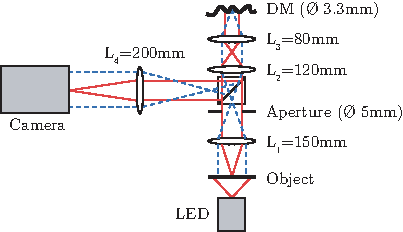
\includegraphics[width=0.50\textwidth]{images/widefield_simple_microscope.pdf}
	\caption{Schematic diagram of the experimental setup, showing a simple microscope complemented with a deformable mirror for aberration correction. Image after~\cite{wide_AOM_loew_freq}.}
	\label{fig:widefield_simple_microscope}
\end{figure}

The presented method uses low spatial frequency content of the image as the optimization metric. The aberration is represented in terms of so called Lukosz modes. Like Zernike polynomials, the Lukosz functions are each expressed as the product of a radial polynomial and an azimuthal function. The presented technique is based on modeling the effects of aberrations on the imaging of low spatial frequencies, which Lukosz modes are are found to be ideal for.

\noindent By modeling the aberration $\Phi(r)$ as a series of $N$ Lukosz modes $L_i(r,\phi)$ with coefficients $a_i$~\cite{wide_Lukosz_Modes}:
\begin{align}
	\Phi(r) = \sum_{i=4}^{N+3}{a_i L_i(r,\phi)},
	\label{eq:aberration_expansion_Lukosz}
\end{align}
they develop the optimization metric $g$ as the sum of a range of low frequencies. It is related to the coefficients of the aberration expansion, $a_i$ by the Lorentzian function~\cite{wide_AOM_loew_freq}
\begin{align}
	g(a_i) \approx \frac{1}{q_0 + q_1 \sum_{i=4}^{N+3}{a_i^2}}
	\label{eq:aberration_metric}
\end{align}
where the piston, tip and tilt modes ($i = 1,2,3$ respectively) have been omitted and $q_0$ and $q_1$ are both positive quantities in the frequency range of interest. The aberration correction process is then performed as the maximization of $g(a_i)$. Because of this particular aberration expansion and  optimization metric, the function $g(a_i)$ shows a paraboloidal maximum that permits the use of simple maximization algorithms. Furthermore, it is shown that the optimization can be performed as a sequence of independent maximizations for each aberration coefficient. 

\begin{figure}[tbh]
			\centering
			\begin{subfigure}[b]{0.8\textwidth}
							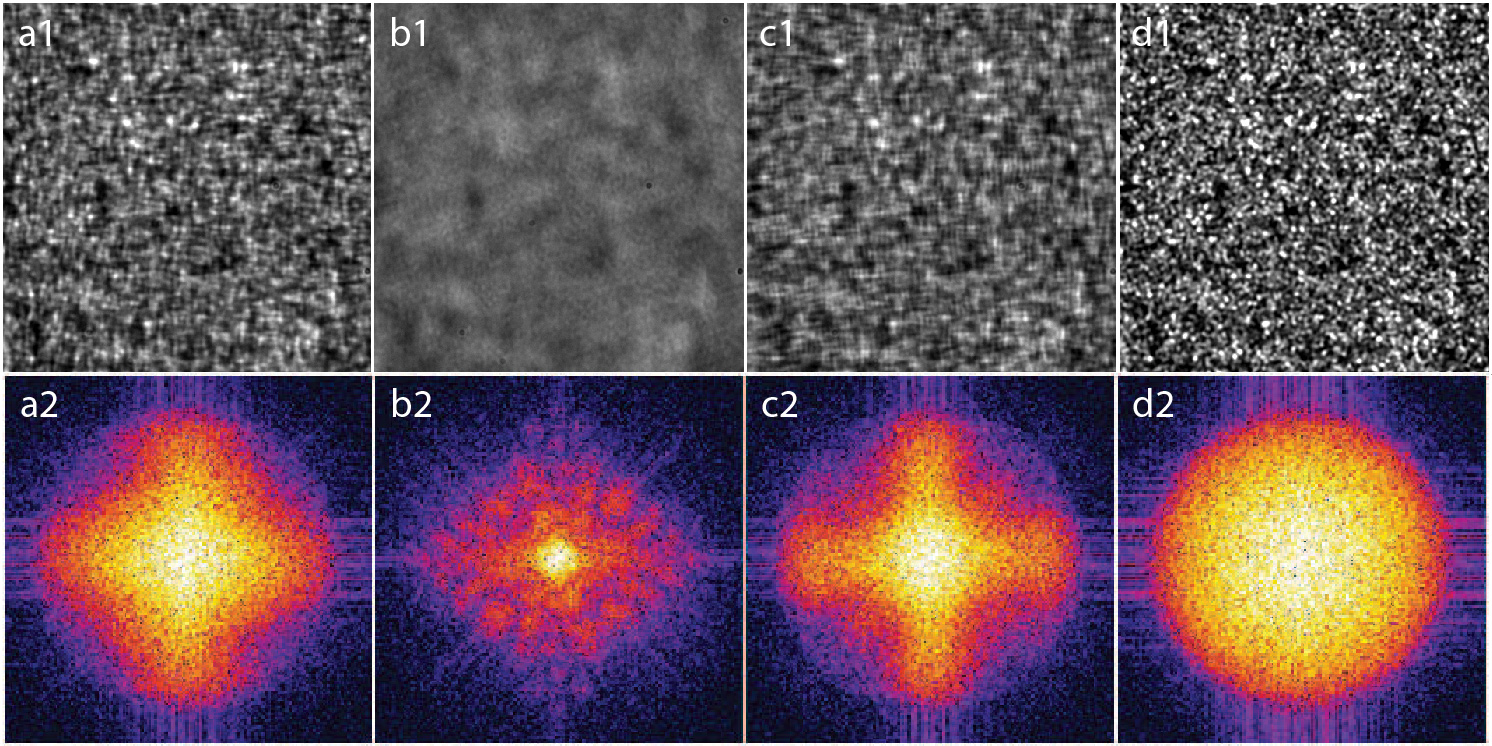
\includegraphics[width=\textwidth]{images/wide_parabolic_opti_images}
							\label{fig:para_opt_images}
			\end{subfigure}
			\begin{subfigure}[b]{0.8\textwidth}
							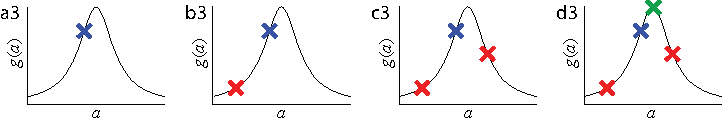
\includegraphics[width=\textwidth]{images/wide_parabolic_opti_graphs}
							\label{fig:para_opt_graphs}
			\end{subfigure}								
			\caption{Correction of a single Lukosz aberration mode (astigmatism, i = 5) for a scatterer specimen and using low spatial frequencies. The first row shows the raw images of the specimen and the second row contains the corresponding spectral densities. The third row illustrates schematically the sampling of the Lorentzian curve used in the optimization calculation. (a1-a3) correspond to an arbitrary initial aberration of magnitude, (b1-b3) have an additional negative bias while (c1-c3) have an additional positive bias of equal magnitude. (d1- d3) show the corrected image calculated with the parabolic minimizationn. Image after~\cite{wide_AOM_loew_freq}.}
	\label{fig:para_opt}
\end{figure} 

The correction process is shown in Figure~\ref{fig:para_opt} for the correction of a single Lukosz mode using a scatterer specimen. Using the deformable mirror (DM), an initial aberration $a_i$ is applied and an image is recorded. The Fourier transform and spectral density of the image are then calculated and the appropriate range of frequency components are summed, giving the metric measurements $g_0$. The same procedure is repeated with both negative and positive aberrations~(i.e. stronger and weaker aberrations), resulting in the metric measurements $g_-$ and  $g_+$. Due to the paraboilc maximum of \eqref{eq:aberration_metric}, the value of $a_i$ that minimizes $g$ can be calculated from as little as three measurements of $g(a_i)$. The optimum correction aberration can then estimated by parabolic minimization as~\cite{wide_parabolic_optimization}:
\begin{align}
	a_\text{corr} = \frac{b(g_+ - g_-)}{2g_+ - 4g_0 + 2g_-}
\end{align}
and is then applied to the DM. To correct multiple modes, each modal coefficient is measured in the same manner before the full correction aberration containing all modes is applied. While this technique is based only on low spatial frequencies, it is shown that both low and high frequency components can be effectively corrected. In all the cases investigated, a Strehl ratio greater than 0.8, close to the diffraction limit, was obtained. This indicates that, when aberration statistics are unknown, choosing small spatial frequencies for an initial correction is a reasonable strategy. If further correction is required,they can be performed using a larger range of frequencies. \emph{Debarre et al.} conclude that this correction scheme is largely independent of the object structure and propose that this approach also to be valid for coherent or partially coherent systems.


%------------------------------------------------------------------------------
\subsubsection{Structured Illumination Microscopy}
\label{sec:StructuredIlluminationMicroscopy}

It is often desired for biological samples to produce clear images of focal planes deep within a thick sample (i.e. optical sectioning) and common techniques include point-scanning techniques such as confocal or multiphoton techniques which are described in Section~\ref{sec:PointScanningMicroscopes}. 

%TODO
Widefield techniques such as Structured Illumination (SI) microscopy can also provide optical sectioning. However, there the sectioning is realized using a standard microscopes, an incoherent light source and without the need for a scanning mechanism. For SI microscopy, a grid is imaged into the specimen to produce a one-dimensional sinusoidal excitation pattern in the focal plane. The resulting sinusoidal fluorescence image, consisting of both in- focus and out-of-focus fluorescence emission, is then normally recorded. Several images are taken, each corresponding to a different grid position equivalent to three different phase shifts of the grating. The grid pattern only appears in the focal plane while it is blurred in the out of focus regions. Hence, it is possible to extract an optical section from the spatially modulated component of the images via a simple calculation.

Based on the SI microscopy technique presented by \emph{Neil et al.} in 2005~\cite{wide_structured_illu_principle} as well as their earlier work on indirect wavefront sensing using a conventional microscope~\cite{wide_AOM_loew_freq} in 2007~(described in the previous section) \emph{Debarre et al.} combined both techniques in 2008 and proposed an AO scheme for use in SI microscopy~\cite{wide_AOM_structured_illu}.  

\begin{figure}
	\centering
		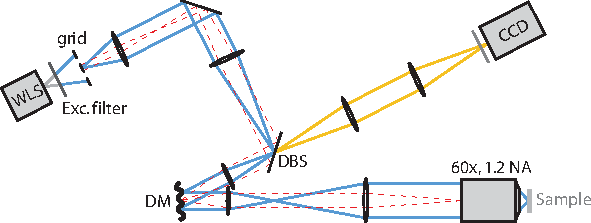
\includegraphics[width=0.75\textwidth]{images/wide_structured_illumination.pdf}
	\caption{Experimental setup for structured illumination microscopy with 
aberration correction. WLS~-~white light source, DM~-~deformable mirror, DBS
~-~dichroic beamsplitter. The blue rays mark the illumination path; the 
detection path is shown in yellow. Image after~\cite{wide_AOM_structured_illu}
.}
	\label{fig:wide_structured_illumination}
\end{figure}

They again present a sensorless wavefront detection scheme, which is shown in Fig.~\ref{fig:wide_structured_illumination}. The method to obtain the aberration correction is similar to the one presented and explained in the previous section. 
The authors derive an inner product from a mathematical model of the imaging process, followed by an orthogonalization process applied to a set of Zernike polynomials. Based on that, a general method providing an optimal aberration expansion for the chosen optimization metric is presented. This process yields  information about the effects of different aberration modes in of the SI microscope. \emph{Debarre et al.} show that the image quality mainly depends on the imaging efficiency spatial frequency of the illumination pattern. This imaging efficiency is affected much more by some aberration modes~(called grid modes) than by others~(called non-grid modes) . Grid modes have a significant influence on the intensity of the sectioned image, whereas non-grid modes have comparatively little effect. The non-grid modes do however affect the resolution. 

The results of the implemented AO scheme is shown in Fig.~\ref{fig:structured_light_correction} for aberration correction on a fluorescent mouse intestine. The image contrast and sharpness improvement is clearly visible in image~\ref{fig:SI_corrected} compared to the uncorrected image in \ref{fig:SI_uncorrected}. As a result of the aberration correction, and as shown in Fig.~\ref{fig:SI_scan}, the contrast of small sample features (blue arrows) is better defined after (red solid line) rather than before (black dotted line) correction. 

\begin{figure}[tbh]
        \centering
        \begin{subfigure}[b]{0.25\textwidth}
                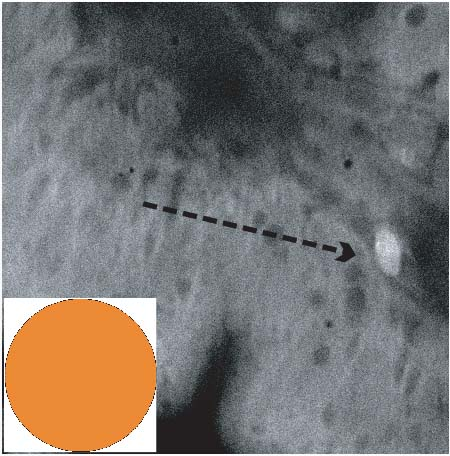
\includegraphics[width=\textwidth]{images/structured_illumination_uncorrected}
                \caption{Uncorrected.}
                \label{fig:SI_uncorrected}
        \end{subfigure}
        \begin{subfigure}[b]{0.25\textwidth}
                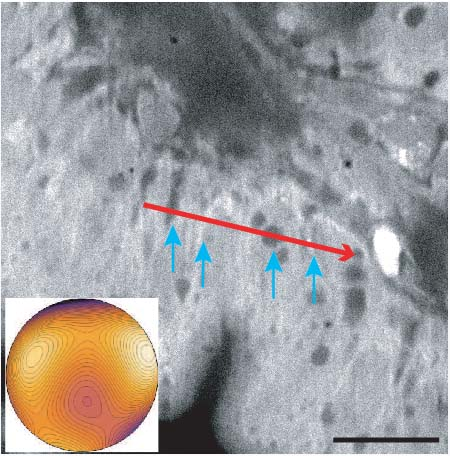
\includegraphics[width=\textwidth]{images/structured_illumination_corrected}
                \caption{Corrected.}
                \label{fig:SI_corrected}
        \end{subfigure}
        \begin{subfigure}[b]{0.25\textwidth}
                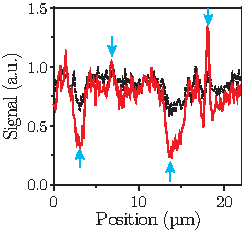
\includegraphics[width=\textwidth]{images/structured_illumination_scan}
                \caption{Line Scan.}
                \label{fig:SI_scan}
        \end{subfigure}
								
        \caption{Aberration correction in structured illumination microscopy. 
A fluorescent mouse intestine sample was imaged (a) without (b) with 
aberration correction with inserts showing the phase induced by the 
deformable mirror. (c) Profile along the lines drawn on the images, both 
profiles normalized so that their mean value is identical. As a result of the 
resolution improvement, the contrast of small sample features (blue arrows) 
is better defined after (red solid line) rather than before (black dotted 
line) correction. The imaging depth was approximately $\unit[10]{\upmu m}$, 
sacle bar size $\unit[10]{\upmu m}$. Image after~\cite{wide_AOM_structured_illu}
.}
\label{fig:structured_light_correction}
\end{figure} 

The authors also explain an additional benefit of aberration correction for structured illumination microscopy. That the adaptive element can also be used to improve the rejection of the out-of-focus fluorescence. When imaging thick specimen, noise fluctuations in the fluorescence signal between the three successive widefield images obtained for the maximization process result in a large out-of-focus background in the calculated sectioned images. Since this background arises from fluorescence generated outside the focal plane, it is not  sensitive to the presence of aberrations. By applying large aberrations in a number of grid modes, the grid pattern is suppressed and only the out-of-focus noise can be measured. By subtracting this aberrated image from the original sectioned image, the fluorescent background can be efficiently removed, leading to greatly improved contrast of the in-focus structures.

The aberrations can also change significantly with depth and hence using the same correction for different depths can result in a degradation of the image quality.  The correction can however be adapted for different imaging depths in the sample. This permits improvement of the image quality throughout an axially extended sample.
It is furthermore possible to determined the appropriate modes once and use the same scheme for any specimen, as the scheme is mostly independent of the object structure. Alternatively, if one wants to correct for local variations in aberrations the image could be formed from several sub-images for which independent aberration correction would be performed.

%TODO is this technique applied in Point Scanning Techniques? 
In conclusion, the authors present a sophisticated, easy to implement and highly versatile AOM scheme which allows for aberration correction induced by the optical system, the specimen or the focus depth. While the presented scheme uses a widefield microscope, \emph{Debarre et al.} are also optimistic that similar AO methods based on indirect, image based aberration detection can be applied to point-scanning methods. 


%------------------------------------------------------------------------------
\subsection{Point Scanning Microscopes}
\label{sec:PointScanningMicroscopes}

Just as with the widefield techniques, adaptive optics quickly found its way into point scanning techniques to improve the image and signal quality. 

Scanning methods are useful for imaging biological specimens, since they can provide high resolution imaging in three-dimensions. Illumination is  usually provided by a laser that is focused into the sample. The light emitted or reflected from the specimen is collected, usually through the same objective lens, and its intensity is measured by a detector. Since this only provides information about the intensity at a single spot, focal point is then scanned through the specimen and point-by-point the image is acquired. 

%ToDo - check what we will actually describe and write short intro for that here...
Several other point scanning microscope modalities have been introduced, including Two-Photon Excitation Fuorescence (TPEF) microscopy, second harmonic generation (SHG) and third harmonic generation (THG) microscopy, and coherent anti-Stokes Raman (CARS) microscopy.

- using a fluorescence microscope, the smaller FWHM, provided by the optimized DMM, will increase the excitation intensity leading to a higher fluorescent signal for the same laser beam input power

3D adaptive optics in a light sheet microscope~\cite{scan_lightSheet}

%------------------------------------------------------------------------------
-
\subsubsection{Confocal Microscopes}
\label{sec:ConfocalMicroscopes}

The most common example of this type is the confocal microscope, which can be 
operated in reflection or fluorescence mode. Three-dimensional resolution is 
achieved by the placement of a pinhole in front of the photodetector. In a 
reflection mode confocal microscope, the illumination is scattered by objects 
not only in the focal region, but throughout the focusing cone. In 
fluorescence mode, emission is generated in the focus but also in out-of-
focus regions. The pinhole ensures that mainly light from the focal region 
falls upon the detector and light from out-of-focus planes is obscured. It is 
critical in the confocal microscope that both the illumination and detection 
paths are diffraction limited. This ensures that i) the illuminating focal 
spot is as small as possible, and ii) that the focus is perfectly imaged on 
to the detector pinhole. Therefore, in an adaptive confocal microscope, 
aberration correction must be included in both paths. This dual pass adaptive 
system can usually be implemented using a single deformable mirror, if the 
path length aberrations are the same for both the illumination and the 
emission light. This is the case if there is no significant dispersion in the 
specimen or chromatic aberration in the optics.

A pinhole is not required to obtain three-dimensional resolution, so most 
TPEF microscopes use large area detectors to maximise signal collection. 
Although they rely upon other physical processes, non-linear imaging 
modalities such as SHG, THG and CARS exhibit similar resolution properties. 
When using large area detectors, the fidelity of imaging in the detection 
path is unimportant so the effects of any aberrations in this path are 
negated. It follows that single pass adaptive optics is appropriate for these 
microscopes as aberration correction need only be implemented in the 
illumination path.

Adaptive optics systems have been successfully combined with several point-
scanning microscope systems including confocal,13 TPEF,6, 14, 15 harmonic 
generation,16, 17 CARS.18 Example images of aberration correction in an 
adaptive THG microscope are shown in Fig. 10.

\cite{book_confocal}
\cite{scan_CFM}

%------------------------------------------------------------------------------
\subsubsection{Two-Photon Fluorescence Microscopy}
\label{sec:twoPhotonExcitation}

Its intrinsic optical sectioning, larger penetration depth, reduced photo damage as well as other advantages allowed nonlinear microscopy in general, and Two-Photon Fluorescence Microscopy~(TPFM) in particular, to become a very important tool in biological imaging since its first presentation by \emph{Denk at al.} in 1990~\cite{scan_TPFM_principle}.

As with most AO microscopy techniques, both a direct and indirect wavefront sensing scheme can be deployed for the use with TPFM. Indirect sensing was already explained~(section~\ref{sec:IndirectWavefrontSensing}) and presented~(section~\ref{sec:WidefieldMicroscopy} in detail. \emph{Marsh et al.} present the first and fairly simple indirect sensing approach, correcting only for depth induced aberrations as early as 2003~\cite{scan_TPFM_pratical}. Again, based on their earlier works~(\cite{wide_AOM_loew_freq,wide_AOM_structured_illu}), \emph{D\'{e}barre et al.} present another highly sophisticated application of their image based wavefront sensing scheme in 2009~\cite{scan_TPFM_image_based}. Both \emph{Marsh} and \emph{D\'{e}barre} essentially use the standard TPFM setup and the image optimization is very similar to the one presented earlier, we will not describe these methods here again.

\emph{Rueckel et al.} present a wavefront correction method using coherence-gated wavefront sensing~\cite{scan_TPFM_gated_wavefront} which also beyond the scope of this report. This section will therefor describe direct wavefront sensing based on the work presented by \emph{Aviles-Espinosa et al.} in 2011~\cite{scan_TPFM_guide_start}.

%rewrite for use here, good general intro....
The resolution has a high dependence on the point-spread function (psf) of the scanned point source. Additionally, the signal levels in two-photon fluorescence have a strong nonlinear dependence upon the incident light intensity. Thus the ideal is to image the sample by use of a diffraction limited spot. However, refractive-index mismatches between the immersion media of high-NA objectives and the sample, in addition to the usually nonuniform samples themselves, impart aberrations to the wavefront and contribute to a deterioration of the psf. Other sources of aberrations include off-axis transmission through optical components, such as the objective and scan lenses while scanning, and imperfections in the optical elements throughout the optical train. The net effect of specimen induced aberrations is that while reducing the achievable resolution, the necessary laser power to achieve imaging increases with depth which can lead to nonreversible effects in biological samples. It also places greater demands in terms of output power on multiphoton imaging laser sources.

%based on \cite{scan_TPFM_guide_start}
- no need to correct on the collected beam as light is only emitted in focus region
- correcting the excitation beam is a must as this will ensure a better focusing and therefore, a more efficient nonlinear (NL) process
- sensor-less schemes, iterative algorithms are generally used to control a deformable mirror (DM) or a Spatial Light Modulator 
- it has been reported the use of optimized algorithms reduce sample exposure
- still implies that an area of interest within the sample has to be exposed a considerable number of times
- may result in unwanted exposure which is prone to produce photo-bleaching and photo-toxic effects on the sample
- We demonstrate that sample induced aberrations can be measured and corrected, 
- In sensor-based schemes  correction performed by measuring aberrations through a wavefront sensor 
- employing a reference point source called guide star
- Then such information is fed to a DM, in order to restore the image quality.
- information is then fed into an adaptive element and aberration is corrected 
- all explained in detail in \ref{sec:WavefrontSensing}
- guide star has been applied for moderate scattering samples imaged through linear fluorescence microscopy~\cite{wide_fluorescence_guide_star} 
- artificially inserting a small, fixed secondary light source inside the sample 
- allows for a direct measurement of the sample aberrations using a Shack-Hartmann (SH) WFS,
- based on the introduction of beads inside the sample 
- it is prone to cause sample damage, limiting its potential for in vivo imaging studies
- beads are randomly distributed inside the fixed sample, suitable bead placed at the right location must be found in the field of view (FOV) and for each depth to be imaged
- adds complexity to the sample preparation and to the aberration measurement process
- Two-photon excited fluorescence (TPEF) naturally produces a small confined volume which can be used as an incoherent secondary light source
- this point source, authors refer to as "`nonlinear guide-star"' (NL-GS), can be used for single pass measurements of sample and objective aberrations
- uses the fact that two-photon excited fluorescence naturally produces a localized point source inside the sample: the nonlinear guide-star (NL-GS).
- The wavefront emitted from the NL-GS can then be recorded using a Shack-Hartmann sensor.
- Compensation of the recorded sample aberrations is performed by the deformable mirror in a single-step. 
- applied to fixed and in vivo biological samples, showing, in some cases, more than one order of magnitude improvement in the total collected signal intensity.
- measured using a WFS placed at the output port of the NLM microscope
- as the WF is directly expressed in the form of Zernike coefficients, it is possible to shape the adaptive element (DM) in a single step (i.e. without the need of any search algorithm) for correcting the measured aberrations
- so, image quality and contrast can be significantly improved without having to expose the sample for large periods of time
- Consequently photo-bleaching and photo-toxicity are greatly reduced
- it can be applied in vivo, it is simple, noninvasive and requires no additional sample processing (such as the incorporation of fluorescent beads)
- Moreover, the NL-GS can be created at any desired position inside a sample
- has been demonstrated with both, moderate and increased scattering samples.
- For moderate scattering samples, when comparing coupling vs. focusing aberrations, we found that the total signal improvement can be up to 11.66 times 
- For samples with increased scattering correction is moderate but in agreement with other adaptive optics correction schemes

\begin{figure}
	\centering
		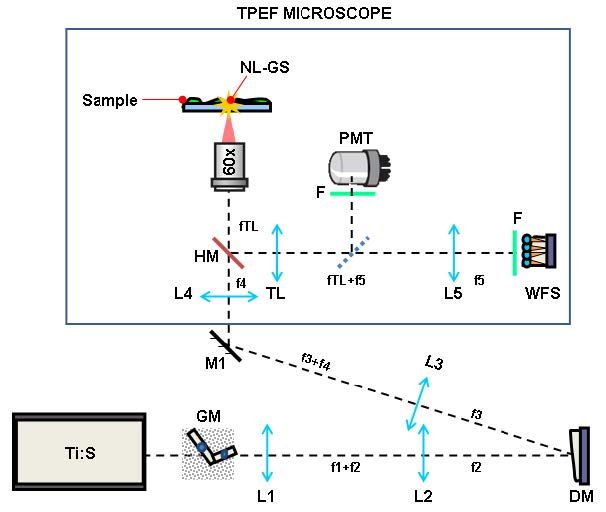
\includegraphics[width=0.75\textwidth]{images/TPFM_guide-star.jpg}
	\caption{check if we really want this...\cite{scan_TPFM_guide_start} Use it...do it yourself and make it nice!!!}
	\label{fig:TPFM_guide-star}
\end{figure}

\cite{scan_TPFM_guide_start}

%------------------------------------------------------------------------------
\subsubsection{Harmonic Generation}
\label{sec:HarmonicGeneration}

\cite{scan_HG_embryos}
\cite{scan_HG_dynamic}


%------------------------------------------------------------------------------
\subsubsection{CARS}
\label{sec:CARS}

\cite{scan_CARS}

%------------------------------------------------------------------------------
\subsubsection{STED}
\label{sec:STED}

\cite{scan_STED}



